\chapter{Background on CMS DAQ System}
\label{Chapter:DAQ}
The Compact Muon Solenoid (CMS) experiment is a particle physics detector built on the proton-proton Large Hedron Collider (LHC) being built at CERN in Switzerland. CMS aims to to explore physics at the electron volt and to discover the Higgs boson. CMS is designed as a general-purpose detector and is going to be capable of studying results of proton collusions to take place inside the LHC. 

An experiment at a hadron collider requires a sophisticated trigger and data acquisition (DAQ) system because of very high collision and overall data rates. The frequency of protons crossing each other at the LHC is 40 MHz \cite{CMSTDR}.

The main goal of the CMS Trigger and Data Acquisition System (TriDAS) is to inspect the detector information at 40 MHz frequency and to select events and to store for offline processing. The events are selected at the maximum rate of $O(10_{2})$. There are two steps in the functionality of the system. The first step, which is called the Level-1 Trigger \cite{CMSTDR}, is designed to reduce the rate of events selected for offline processing to less than 100 kHz. The second step, which is called High-Level Trigger (HLT), is designed to further reduce the 100 kHz. of the Level-1 Trigger to the final output rate of 100 Hz. 

Functionality of the CMS DAQ and HLT is given in the CMS DAQ Technical Design Report as follows \cite{CMSTDR}:

\begin{itemize}
	\item ``perform the readout of the front-end electronics after a Level-1 Trigger accept''
	\item ``execute physics selection algorithms on the events read out, in order to accept the ones with the most interesting physics content''
	\item ``forward these accepted events, as well as a small sample of rejected events, to the online services which monitor the performance of the CMS detector and also provide the means of archiving the events in mass storage''
\end{itemize}

Figure \ref{fig:triggerdaq} shows the data flow in the Trigger/DAQ system and also visualizes the Level-1 Trigger and HLT stages mentioned above.

\begin{figure}
	\centering
		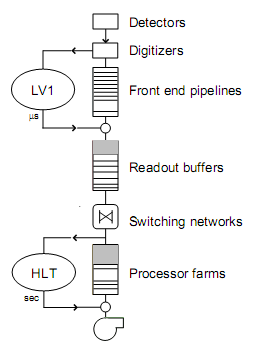
\includegraphics[width=0.45\textwidth]{figures/triggerdaq.png}
	\caption{Data Flow in the Trigger/DAQ System}
	\label{fig:triggerdaq}
\end{figure}

\section{DAQ Architecture}
Figure \ref{fig:xdaqarch} shows the architecture of the CMS DAQ system. The system consists of the following elements:

\begin{itemize}
	\item \textbf{Detector Front-ends} are the components that are connected to the front-end electronics to store the data from them as the Level-1 Trigger accept signal is received. 
	\item \textbf{Readout Systems} are the components that are connected to the Front-End System (FES) to read the data from the detector. Readout systems store the data until they are sent to the processor to which will analyze the event.There are about 500 components which are called ``Readout Columns''. Each Readout Column consists of a number of Front-End Drivers (FEDs) and one Readout Unit (RU). RU is responsible for keeping the event data in its buffer and interfacing to the switch.
	\item \textbf{Builder Network} is a collection of networks providing the interconnections between the Readout and Filter Systems. It can handle 800Bg/s sustained throughput to the Filter Systems.
	\item \textbf{Filter Systems} are the processors that the RUs provide the events with. Filter systems are the entities that decide whether a supplied event is interesting and will be kept for offline processing or not. The interestingness of an event is determined by executing the High-Level Trigger algorithms. There are about 500 entities which are called ``Filter Columns''. Each of those include one Builder Unit (BU). A BU is responsible for receiving incoming data fragments that correspond to a single event and building them into full event buffers. 
	\item \textbf{Event Manager} controls the flow of events in the system. Event Manager (EVM) serves as a centralized intelligence of event management.
	\item \textbf{Computing Services} are composed of all the processors and networks that receive filtered events and some of the rejected events from the Filter Farms.
	\item \textbf{Controls} are responsible for the user interface and the configuration and monitoring of the DAQ.
\end{itemize}

\begin{figure}
	\centering
		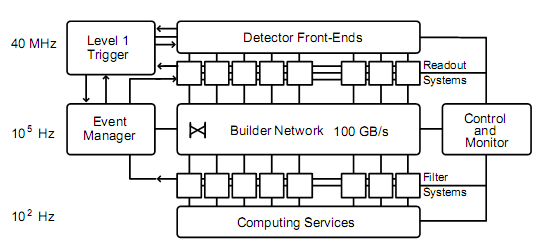
\includegraphics[width=0.90\textwidth]{figures/xdaqarch.png}
	\caption{CMS DAQ System Architecture}
	\label{fig:xdaqarch}
\end{figure}

Given the component breakdown of the system it is possible to identify four stages of system functionally. First stage is a detector readout stage where events are collected and stored in buffers. The second stage is the event building stage, where all data corresponding to a single event are collected from the buffers. The third stage is the selection stage where High-Level Trigger in the processor processes the event. The final stage is the analysis and storage stage where the events that are selected in the previous stage are sent to the Computing Services for additional processing for storage or further analysis. 

XDAQ uses a format called I20 data binary data format. I2O (Intelligent Input Output) is an I/O architecture specification developed by a consortium of computer companies called the I2O special Interest Group (SIG) for managing devices. The details of the I2O message format is not in the scope of this research. However, more information about the details of the I2O specification may be obtained from \cite{I2O}.


\section{Event Builder}
The main task of the DAQ system is to read each event's corresponding data out of the FEDs and merge it into the single structure called ``physics event'' and to transmit the physics event to a filter farm consisting of processor that execute physics algorithms that decide whether the event should be kept for further processing or discarded \cite{CMSTDR}. The Event Builder (EVB) is the central component of the DAQ system and includes the components that are responsible for this task.

Figure \ref{fig:builder} shows a more detailed version of the DAQ architecture depicted in Figure \ref{fig:xdaqarch}.

\begin{figure}
	\centering
		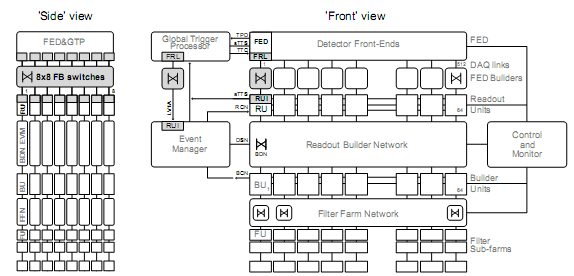
\includegraphics[width=0.90\textwidth]{figures/builder.png}
	\caption{Front and Side Views of the DAQ}
	\label{fig:builder}
\end{figure}

In the first of the stages that were idenfied above, there exist 8 FEDs that the RUs read data from and perform merging of event data fragments into larger data blocks called ``super-fragments'' or ``s-fragments''. This arrangement makes up a 64 ``FED Builders'' each of which consists of 8 FEDs, a 8x8 switch, and 8 RUs. Readout data is distributed among 64 RUs to maximize readout bandwidth. Thus, parts of data from a single event are buffered in 64 RUs. In the second state, 64 BUs which read out the data from a single event contained in 64 RUs and build these 64 s-fragments to form a single event. RUs and BUs are connected to each other through a 64x64 switch. The group of 64 RUs, the 64x64 switch and 64 BUs are called the ``RU Builder''. The full XDAQ system is composed of 64 FED Builders and 8 RU Builders. Figure \ref{fig:3dxdaq} shows the three-dimensional representation of the system \cite{CMSTDR}.

\begin{figure}
	\centering
		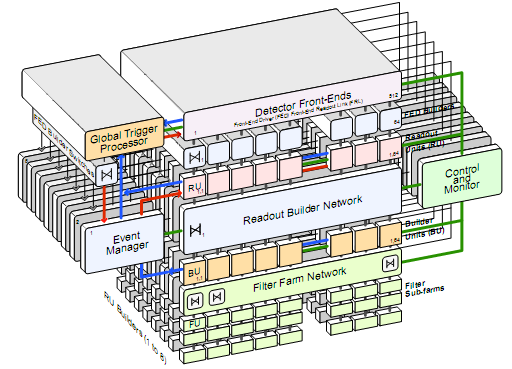
\includegraphics[width=0.90\textwidth]{figures/3dxdaq.png}
	\caption{Three-Dimensional View of the System}
	\label{fig:3dxdaq}
\end{figure}



\section{RU Builder}

This research is mainly interested in the components of the RU Builder as the experimental platform. Figure \ref{fig:evbsystem} shows the event builder and how the RU Builder is connected to the rest of the system \cite{rubuilder}. 

RU Builder consists of several applications. There is a single Event Manager (EVM), one or more readout units (RUs), and one or more builder units (BUs). The trigger adapters (TAs), readout unit inputs (RUIs) and filter units (FUs) are external to the RU Builder and are not in the scope of the experimental platform of this research. 

\subsection{Event Manager (EVM)}
EVM is the application that controls the flow of event data through the RU Builder. Figure \ref{fig:evm} shows the internal FIFOs of the EVM and its dynamic behavior.

In the first step, EVM receives trigger data of an event from the RUI. In step 2, EVM assigns a free event ID to the trigger data. In step 3, EVM requests the RUs to readout the event's data. In step 4, BU asks the EVM to allocate it an event. In this request, BU may also send an event ID to be cleared. In step 5, EVM saves the event ID received from BU as a free ID. In step 6, EVM sends the BU a confirmation of the allocation by sending the requesting BU the assigned event ID and trigger data of the allocated event. \cite{rubuilder}

\begin{figure}
	\centering
		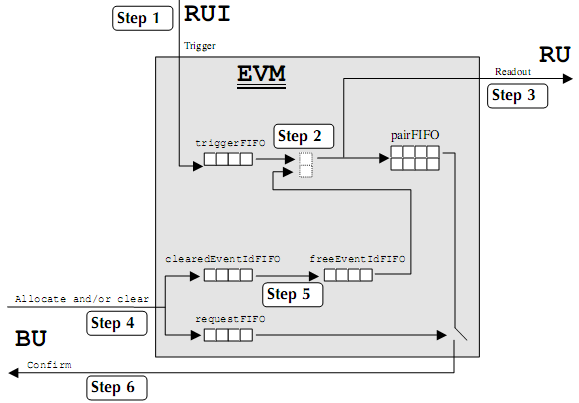
\includegraphics[width=0.90\textwidth]{figures/evm.png}
	\caption{Dynamic Behavior of EVM}
	\label{fig:evm}
\end{figure}

\subsection{Readout Unit (RU)}
RU is the application that buffers the s-fragments until there is a BU request. Figure \ref{fig:ru} shows the internal FIFOs of the RU and its dynamic behavior.

\begin{figure}
	\centering
		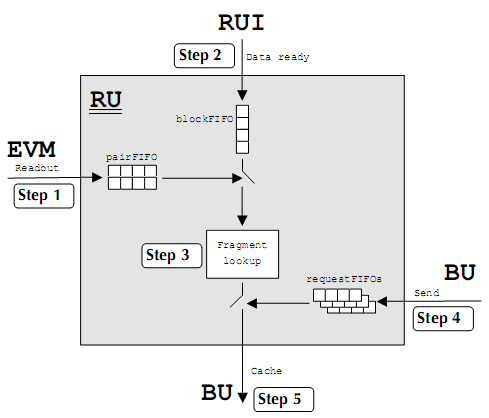
\includegraphics[width=0.90\textwidth]{figures/ru.png}
	\caption{Dynamic Behavior of RU}
	\label{fig:ru}
\end{figure}

In the first step, RU receives a pair of ``event ID/trigger event number'' and asks the RU to readout the data of the assigned event ID. In step 2, RUI tells the RU that event's data is ready to for readout and processing. In step 3, a RU fills in its fragment lookup table with each s-fragment for which it received pair for from the EVM. In step 4, BUs request from RUs the s-fragments of the events that they received confirmation for from the EVM. In step 5, a RU fulfills the request from a BU with s-fragments retrieved from the s-fragment from its fragment lookup table and asks the BU to cache the events data \cite{rubuilder}.

\subsection{Builder Unit (BU)}

BU is the application that is responsible for event building. Figure \ref{fig:bu} shows the internal FIFOs of the RU and its dynamic behavior.

\begin{figure}
	\centering
		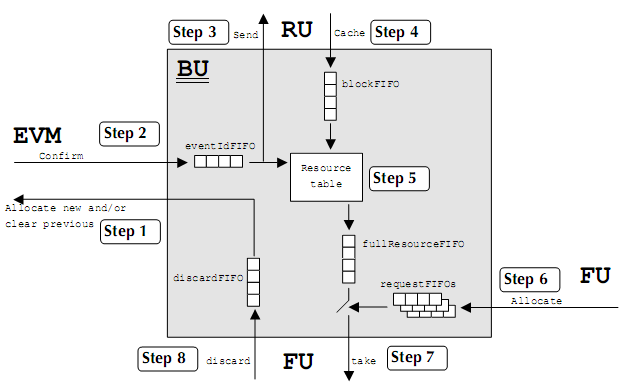
\includegraphics[width=0.90\textwidth]{figures/bu.png}
	\caption{Dynamic Behavior of BU}
	\label{fig:bu}
\end{figure}

In the first step, the BU with free capacity asks the EVM to allocate it an event. In step 2, BU receives the confirmation of event allocation from the EVM along with the event ID and trigger data of an event which makes up the first s-fragment of the event. In step 3, the BU asks the RUs for the rest of the event's s-fragments. In step 4, the BU receives the the rest of the event's s-fragments from RUs, and caches them in its block FIFO. In step 5, the BU builds the event's s-fragments into one whole event in its resource table. In step 6, FUs requests an event from BU for processing. In step 7, BU allocates a whole event to the requesting FUs. In step 8, when a FU finishes processing an event, it asks BU to discard the event ID corresponding to processed event \cite{rubuilder}.

\section{Summary}
CMS DAQ system is the data acquisition system for the CMS experiment. In this chapter, basic information about the architecture of the CMS DAQ system was given. The focus was given on the Event Builder and more specifically the RU Builder and its applications. RU Builder applications are used as part of the experimental platform for this research. 